\textit{ Consider the simple relay system given in the following figure. S sends the packet 
to R at the rate $R_1$ and then R forwards that data to D by using data rate $R_2$. Derive the 
equivalent end—to—end rate between S and D. }

\begin{figure}[!h]
  \centering
  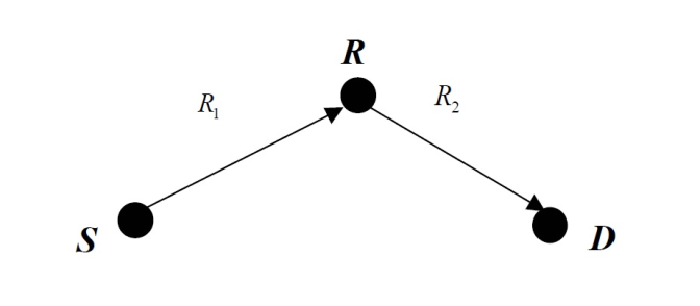
\includegraphics[width=8cm]{multiagent_2-jpg.eps}
  \caption{Relay retransmission}
  \label{fig:multiagent_2-jpg}
\end{figure}

Assuming that the rate is given in symbols/second or bits/second then the equivalent transmission rate from S to D must be the minimum between the two rates ($R_1$,$R_2$), as shown in \figref{fig:multiagent_2-jpg}. This is based on the assumption that the node R always relays the transmitted packages from S to D.